
\documentclass[a4paper,UKenglish,cleveref, autoref]{oasics-v2019}
%This is a template for producing OASIcs articles. 
%See oasics-manual.pdf for further information.
%for A4 paper format use option "a4paper", for US-letter use option "letterpaper"
%for british hyphenation rules use option "UKenglish", for american hyphenation rules use option "USenglish"
%for section-numbered lemmas etc., use "numberwithinsect"
%for enabling cleveref support, use "cleveref"
%for enabling cleveref support, use "autoref"

\usepackage{fancyvrb}
\VerbatimFootnotes

%\graphicspath{{./graphics/}}%helpful if your graphic files are in another directory

\bibliographystyle{plainurl}% the mandatory bibstyle

\title{Opening Digitized Newspapers Corpora: Europeana’s Full-text Data Interoperability Case} %Please add

\titlerunning{Opening Digitized Newspapers Corpora}%optional, please use if title is longer than one line

\author{Nuno Freire}{INESC-ID, Lisbon, Portugal}{nuno.freire@tecnico.ulisboa.pt}{https://orcid.org/0000-0002-3632-8046}{}%mandatory, please use full name; only 1 author per \author macro; first two parameters are mandatory, other parameters can be empty. Please provide at least the name of the affiliation and the country. The full address is optional

\author{Antoine Isaac}{Europeana Foundation, The Hague, The Netherlands}{antoine.isaac@europeana.eu}{https://orcid.org/0000-0001-9767-6979}{}
\author{Twan Goosen}{CLARIN ERIC, Utrecht, The Netherlands}{twan@clarin.eu}{https://orcid.org/0000-0002-1634-257X}{}
\author{Daan Broeder}{KNAW Humanities Cluster, Amsterdam, The Netherlands}{daan.broeder@di.huc.knaw.nl}{https://orcid.org/0000-0002-8446-3410}{}
\author{Hugo Manguinhas}{Europeana Foundation, The Hague, The Netherlands}{hugo.manguinhas@europeana.eu}{}{}
\author{Valentine Charles}{Europeana Foundation, The Hague, The Netherlands}{valentine.charles@europeana.eu}{https://orcid.org/0000-0003-4085-5778}{}

\authorrunning{N. Freire, A. Isaac, T. Goosen, D. Broeder, H. Manguinhas and V. Charles} %\authorrunning{J.\,Q. Public and J.\,R. Public}%mandatory. First: Use abbreviated first/middle names. Second (only in severe cases): Use first author plus 'et al.'


\Copyright{Nuno Freire, Antoine Isaac, Twan Goosen, Daan Broeder, Hugo Manguinhas and Valentine Charles}%mandatory, please use full first names. OASIcs license is "CC-BY";  http://creativecommons.org/licenses/by/3.0/

\ccsdesc[300]{Applied computing~Digital libraries and archives}
\ccsdesc[100]{Applied computing~Annotation}
\ccsdesc[100]{Applied computing~Document metadata}
%mandatory: Please choose ACM 2012 classifications from https://dl.acm.org/ccs/ccs_flat.cfm 

\keywords{Metadata, Full-text, Interoperability, Data aggregation, Cultural Heritage, Research Infrastructures}%mandatory; please add comma-separated list of keywords

%\category{}%optional, e.g. invited paper

%\relatedversion{}%optional, e.g. full version hosted on arXiv, HAL, or other respository/website
%\relatedversion{A full version of the paper is available at \url{...}.}

%\supplement{}%optional, e.g. related research data, source code, ... hosted on a repository like zenodo, figshare, GitHub, ...

%\funding{(Optional) general funding statement \dots}%optional, to capture a funding statement, which applies to all authors. Please enter author specific funding statements as fifth argument of the \author macro.

%\acknowledgements{I want to thank \dots}%optional

%\nolinenumbers %uncomment to disable line numbering

%\hideOASIcs  %uncomment to remove references to OASIcs series (logo, DOI, ...), e.g. when preparing a pre-final version to be uploaded to arXiv or another public repository

%Editor-only macros:: begin (do not touch as author)%%%%%%%%%%%%%%%%%%%%%%%%%%%%%%%%%%
\EventEditors{John Q. Open and Joan R. Access}
\EventNoEds{2}
\EventLongTitle{42nd Conference on Very Important Topics (CVIT 2016)}
\EventShortTitle{CVIT 2016}
\EventAcronym{CVIT}
\EventYear{2016}
\EventDate{December 24--27, 2016}
\EventLocation{Little Whinging, United Kingdom}
\EventLogo{}
\SeriesVolume{42}
\ArticleNo{23}
%%%%%%%%%%%%%%%%%%%%%%%%%%%%%%%%%%%%%%%%%%%%%%%%%%%%%%

\begin{document}

\maketitle

%mandatory: add short abstract of the document
\begin{abstract}
Cultural heritage institutions hold collections of printed newspapers that are valuable resources for the study of history, linguistics and other Digital Humanities scientific domains. Effective retrieval of newspapers content based on metadata only is a task nearly impossible, making the retrieval based on (digitized) full-text particularly relevant. Europeana, Europe’s Digital Library, is in position to provide access to large newspapers collections with full-text resources. Full-text corpora are also relevant for Europeana’s objective of promoting the usage of cultural heritage resources for use within research infrastructures. We have derived requirements for aggregating and publishing Europeana’s newspapers full-text corpus in an interoperable way, based on investigations into the specific characteristics of cultural data, the needs of two research infrastructures (CLARIN and EUDAT) and the practices being promoted in the International Image Interoperability Framework (IIIF) community. We have then defined a `full-text profile' for the Europeana Data Model, which is being applied to Europeana’s newspaper corpus.
\end{abstract}

\section{Introduction}
\label{sec:introduction}
Cultural Heritage Institutions (CHIs), such as libraries and archives, hold collections of printed newspapers of the past centuries. These are valuable resources for historians, linguists and other researchers working in Digital Humanities. The retrieval of printed newspapers' content based on metadata only is a task nearly impossible, however. CHIs usually describe the series of a newspaper publication (typically known as `title level' description) and its individual publications (`issues') in their catalogs, but no description of individual articles. The typical use of the catalogs of newspapers is thus only to retrieve issues by date of publication, as there is no detail for effective retrieval of the content at finer-grained levels. 

The wide interest for newspapers and the challenges they pose for retrieval has motivated CHIs to prioritize the digitization of their newspapers collections. CHIs also realized that the retrieval of newspapers' content based on machine readable full-text is particularly important, given the unavailability of article level descriptions in the catalogs. Accordingly, CHIs have also sought to apply Optical Character Recognition (OCR) during the digitization process.  

Our work addresses the general problem of the retrieval of newspapers in the context of aggregations of digital CH resources, in particular that of Europeana. Europeana seeks to facilitate the use of resources from and about Europe. It enables access to objects via its Collections portal
\footnote{\url{https://europeana.eu}}, which supports all official languages of Europe, and its open APIs enable third-party applications. Europeana is based on metatada provided by its CHI partners and presently holds metadata from over 3,700
CHIs\footnote{\url{https://pro.europeana.eu/files/Europeana_Professional/Projects/Project_list/Europeana_DSI/Deliverables/europeana-dsi-d1.2-amount-of-data-partners-and-outreach-to-major-institutions.pdf}}.
Providing access to newspapers is relevant to Europeana's mission, especially for promoting the re-use of CH resources for research. Europeana indeed also aims to facilitate research, especially for the digital humanities, via its Europeana Research
initiative\footnote{\url{https://research.europeana.eu}}.
This initiative seeks to address issues related to, e.g., licensing, which affect the research re-use of CH metadata and content. In particular, it has identified research re-use of newspapers resources as a key use case, as well as an area with strong system and data interoperability challenges.

Digitized newspapers are Europeana's first case of aggregation and distribution of full-text CH resources. Europeana's systems have relied so far on metadata and links to digitized resources at partners' sites. The Europeana Data Model (EDM) \cite{edm} allows it to perform scalable aggregation of (and access to) references to digital representations of CH artefacts with rich context metadata. EDM follows the Linked Open Data principles \cite{BernersLee06}. An important aspect of EDM is its flexibility and genericity: it can be easily mapped to other (CH) data models and extended \cite{Charles15}. This makes it a potential base for the interoperability of full-text resources within the Europeana ecosystem.

This paper presents how we have tested this assumption by trying to extend EDM to cater for interoperability of full-text CH corpora. The first aim of our work is to support a centralized search engine and rich user interfaces. But we have also investigated the issue of interoperability of full-text between Europeana and research infrastructures (EUDAT and CLARIN). Our work focuses on Europeana and research use, but we claim it has impact on other application contexts, as we sought to align with the generic International Image Interoperability Framework
(IIIF)\footnote{\url{https//iiif.io}}. 
We present related work on digitized newspapers and the use of CH data in research infrastructures in Section~\ref{sec:relatedwork}. Section~\ref{sec:needsforinteroperability} presents the explorative work conducted by Europeana, EUDAT and CLARIN, and the interoperability requirements derived from it. Section~\ref{sec:buildingfulltextprofile} presents our EDM extension for full-text, and Section~\ref{sec:conclusion} concludes. 

\section{Related work}
\label{sec:relatedwork}

Several initiatives exist worldwide with similar target user groups and use cases as Europeana, with respect to aggregation of digitized newspapers. The organizational structure and technical interoperability context of Europeana are quite different, however. For example, Chronicling 
America\footnote{\url{https://chroniclingamerica.loc.gov/}}, a national aggregation of newspapers in the US, gathers its corpus from the digitization conducted under the National Newspaper Digitization Program. The direct relation with the digitization process results in more homogeneous metadata and full-text content to provide access to.

Europeana Newspapers \cite{Dunning15} was an earlier project from the Europeana community, which aggregated metadata and full-text content in a portal that, while currently hosted by Europeana, sits on a completely disconnected platform. The project established interoperability by defining a METS/ALTO profile \cite{Muehlberger14}, but its application was restricted to the project and did not spread to other CHIs afterwards.

The IIIF Community has conducted similar work to ours in establishing a generic representation of full-text associated with images for the IIIF Presentation API. We participate in a IIIF Newspapers Community Group that gathers IIIF community members working with digitized newspapers. We got a lot of inspiration from the IIIF representation patterns. These are quite generic however and the connection with (descriptive) metadata is rather loose in the IIIF presentation API, which relies on linking to document using models like EDM for representing fully-fledged metadata. Furthermore, directly relying on IIIF APIs is an obstacle for the metadata providers who cannot deploy IIIF services for their content.

Regarding interoperability with research infrastructures, related work in CH digitized resources and OCR full-text includes Herbadrop \cite{Dugenie2017}. This initiative works with resources from museums and botanical gardens, which own collections of plant samples with detailed annotations from botanists. Herbadrop has worked with the EUDAT 
CDI\footnote{EUDAT Collaborative Data Infrastructure; \url{https://www.eudat.eu/eudatcdi}}
as part of a data pilot \cite{Dugenie2017}. 

Finally, some CHIs provide data to 
CLARIN\footnote{Common Language Resources and Technology Infrastructure; \url{https://www.clarin.eu/}},
in particular university libraries. CLARIN aggregates CH resources in a similar process to Europeana's but uses a different metadata format \cite{cmdi}. Regarding full-text corpora within CLARIN, we observe a prevalence of the Text Encoding Initiative (TEI)
format\footnote{TEI -- Text Encoding Initiative; \url{https://www.tei-c.org/}}
in terms of support by existing tools and also in published research. TEI usage within the Europeana Network is limited: it is only present in CHIs that focus on supporting researchers. 

\section{Needs for interoperability with Research Infrastructures}
\label{sec:needsforinteroperability}
Europeana is interested in investigating how research data infrastructures can facilitate the research use of CH resources. By leveraging on European level and cross-discipline infrastructures, it hopes to reach researchers from all scientific disciplines, without having to work with many national and domain-specific research infrastructures or providing its own. We describe here the efforts on the Europeana Newspapers corpus conducted with two infrastructures: CLARIN and EUDAT. This corpus was aggregated from 11 CHIs during the Europeana Newspapers project. It contains metadata descriptions, digitized images and full-text of 911 newspaper titles that, in total, comprise over 11 million pages \cite{Dunning15}. We present, in this section, the interoperability challenges identified and what we did to tackle them. 

\subsection{Interoperability with CLARIN}
\label{sec:interoperabilitywithclarin}
CLARIN is a federation of language data repositories, service centers and centers of expertise. CLARIN aggregates metadata and makes the underlying resources discoverable and usable within research workflows. It allows researchers to carry out natural language processing tasks by invoking processing tools directly from its generic user interface. Establishing good interoperability between Europeana and CLARIN can help fitting a large number of CH resources into CLARIN's supported workflows. It will open up new applications for CLARIN's processing tools and greatly promote research incorporating CH resources.

CLARIN carried out a first analysis of the Europeana Newspapers corpus in 2015, establishing goals and a ground for connecting the two infrastructures and full-text interoperability. Later, we sought to address the interoperability issue for metadata \cite{Goosen17}. The two infrastructures use specific metadata models: EDM for Europeana and the Component MetaData Infrastructure (CMDI) for CLARIN \cite{cmdi}. Interoperability is achieved via CLARIN's metadata conversion mechanisms, based on a CMDI profile for 
EDM\footnote{Available in CLARIN’s component registry:  \url{https://catalog.clarin.eu/ds/ComponentRegistry/##/?itemId=clarin.eu\%3Acr1\%3Ap_1475136016208}}.
Europeana's metadata for Newspapers and other datasets can thus be made available within the CLARIN systems. 

The desirable interoperability between the two infrastructures has not been achieved, however. The Newspapers full-text corpus, although discoverable within CLARIN, cannot yet be processed by CLARIN's tools in research workflows. The following requirements for how metadata and full-text content are made available by CHIs were noted and greatly influenced our work on extending EDM for exchanging full-text content:
\begin{itemize}
\item Direct links to content files – when CHIs only share with Europeana links to websites or viewers, the files cannot be processed by CLARIN (and others).
\item Technical metadata – information like media type and file size are essential for automated processing workflows and highly desirable for discovery
\item Language of the content – most natural language processing tools are language dependent, making the language information carried in CH metadata essential.
\end{itemize}

\subsection{Interoperability with EUDAT}
\label{sec:interoperabilitywitheudat}
EUDAT is a European infrastructure of integrated data services devoted to scientific and research data storage and lifecycle management. It has been developed in close collaboration with over 50 research communities spanning across many different scientific disciplines such as Life Sciences, Humanities, Earth Sciences and Physics, with more than 20 major European research organizations, data centres and computing centres involved. Many of these collaborations are carried out as data pilots providing test-beds that vary in disciplines, communities, project group sizes and technological maturity. Europeana conducted a data pilot with EUDAT that consisted in a case study on the Europeana Newspapers corpus \cite{Dugenie2017}. The general goal was to investigate how EUDAT data services can facilitate the use of CH resources for research purposes. The questions laid out at the start of the data pilot were:
\begin{itemize}
\item How can the resources be discovered?
\item How can the resources be shared in practical ways for researchers? 
\item How can advanced computation be applied to these CH datasets? 
\item How can the resources and datasets be cited and referenced in research?
\item How can the CH institutions re-use the outcomes of research?
\end{itemize}

An evaluation of the available EUDAT services was conducted, using the newspapers corpus as case study. The two infrastructures were successfully interconnected and EUDAT fulfilled the expectations for making the corpus available to researchers and for computational processing. The persistent identification of EUDAT resources also met the citability requirement. The EUDAT service did not scale to the dimension of the corpus, but only due to an underestimation of the required computational capacity during the pilot \cite{Dugenie2017}. Beyond the full-text corpus case study, interoperability was also trialled for metadata-based discovery of CH datasets. Both infrastructures have common underlying technologies that facilitate interoperability, including on modelling full-text, since EUDAT is developing its semantic annotation service based on the W3C Web Annotation Data 
Model\footnote{\url{https://www.w3.org/TR/annotation-model/}},
which is a key component of the EDM extension we are going to present in the next section.

\section{Building a full-text profile for the Europeana Data Model}
\label{sec:buildingfulltextprofile}

A profile for representing full-text in EDM is a key requirement for achieving a sustainable interoperability framework for full-text CH corpora in Europeana. It has potential applications in full-text aggregation, indexing, user experience and data re-use. This section presents the context, requirements and the EDM full-text profile.

\subsection{Context and requirements for designing the data model}
\label{sec:contextandrequirements}

Based on the corpus of full-text newspapers, the case studies and recommendations from the earlier Europeana projects \cite{Dunning15, Charles16}, we have identified these requirements:
\begin{itemize}
\item The availability of full-text must be stated explicitly in the metadata.
\item The representation of full-text should be compatible with the representation of structured newspapers in the descriptive metadata.
\item URLs to views of the digital objects must be explicitly stated in the metadata.
\item Multiple full-text resources must be referenced via direct URLs. 
\item Resources requiring a protocol to be served need to be clearly identifiable.
\item When more than one full-text resource is associated with a digital object, it should be possible to represent their part-whole relationship. 
\item When more than one full-text resource is associated with a digital object, it should be possible to represent their sequential order. 
\item When a full-text resource is available as a fragment of text, the URI or the literal identifying the specific text fragment may be provided in the data.
\item When a full-text fragment is available, the image area it refers to should be identified (via coordinates).
\end{itemize}

The IIIF community has suggested to publish textual representations of (part of) images, such as transcriptions, using annotations from the W3C Web Annotation model (WA). Annotations are included in the IIIF
`manifests'\footnote{IIIF manifests are `the overall description of the structure and properties of the digital representation of an object.'; \url{http://iiif.io/api/presentation/2.0/##primary-resource-types}}
of the newspapers, as a list of annotations, each one referring to a portion of the full-text and indicating its corresponding position in the image of a page. Representing full-text as annotations seems the best solution as it can support simple scenarios such as the positioning of a text fragment on an image as well as more complex ones like OCR correction.

This approach, besides its community traction, is compatible with the Linked Data vision and fits well Europeana's use of annotations for other purposes \cite{Gordea15}. One of the cases that has recently emerged in Europeana is indeed the representation of manual transcriptions of content\footnote{Cf.\, Europeana’s initiative on transcribing WWI-related content; \url{https://transcribathon.com/}}.
As meeting the requirements of these related cases in similar ways is extremely desirable, we decided to follow the IIIF Community approach. Our modelling exercise thus becomes one of fitting into EDM a representation of the full-text content of newspapers as annotations on the images of newspapers' pages. 

\subsection{EDM extension addressing the initial full-text requirements}
\label{sec:edmextension}

\begin{figure}
    \centering
    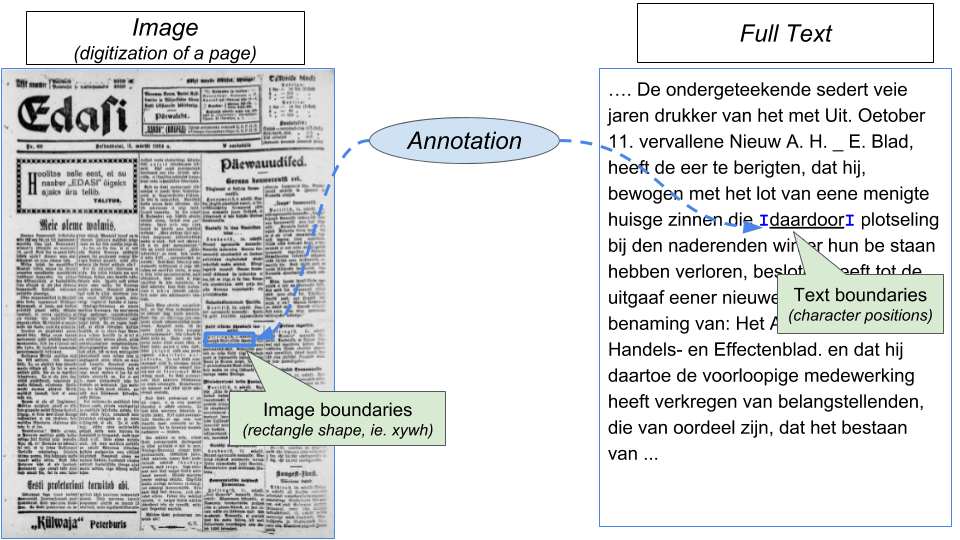
\includegraphics{Fig1}
    \caption{General principles for full-text annotations in the EDM extension.}\label{fig:generalprincipals}
\end{figure}

Our extension of EDM for representing full-text follows the recommendations of IIIF (in its coming version 3) and WA. Full-text is represented as the body of an annotation that has as target an image, as illustrated in Figure~\ref{fig:generalprincipals}. We model the image as an \verb+edm:WebResource+ (the usual EDM approach) and the text itself as a new proposed subclass of \verb+edm:WebResource+, 
\verb+edm:FullTextResource+\footnote{The full-text comes as \verb+rdf:value+ for the \verb+edm:FullTextResource+, using WA’s `embedded text' pattern (\url{https://www.w3.org/TR/annotation-model/##embedded-textual-body}) with a type independent from the resource’s being used in an annotation, unlike WA’s \verb+oa:TextualBody+.}.
Figure~\ref{fig:nopositioninfo} illustrates the simplest case. Annotations are modeled using WA's \verb+oa:Annotation+ class and \verb+oa:hasBody+ and \verb+oa:hasTarget+ properties. Annotations used for representing full-text must have the property \verb+oa:motivatedBy+ with the value \verb+oa:transcribing+, distinguishing them from Europeana annotations used for other motives, as well as following IIIF's latest best practices\footnote{Cf.\, IIIF API issue 1258: \url{https://github.com/IIIF/api/issues/1258}}
(NB: we omit it from our figures for readability reasons).

The extension supports two levels of detail for associating the full-text with the image: with and without its position within the image. The text can also be provided by value (a plain literal) or by reference (as a URI, and/or as a selection/extract from another text resource). The following sections present the details of these options.

\subsubsection{Full-text without position}

\begin{figure}
    \centering
    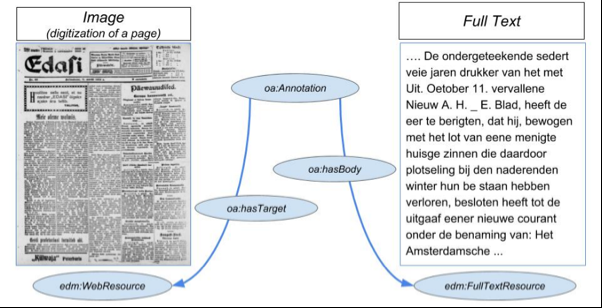
\includegraphics{Fig2}
    \caption{Full-text without position information.}\label{fig:nopositioninfo}
\end{figure}

In the simplest case, illustrated in Figure~\ref{fig:nopositioninfo}, full-text is associated with an image without any information about the position of the text within the image.

\subsubsection{Full-text associated with fragments with a position in the image}

\begin{figure}
    \centering
    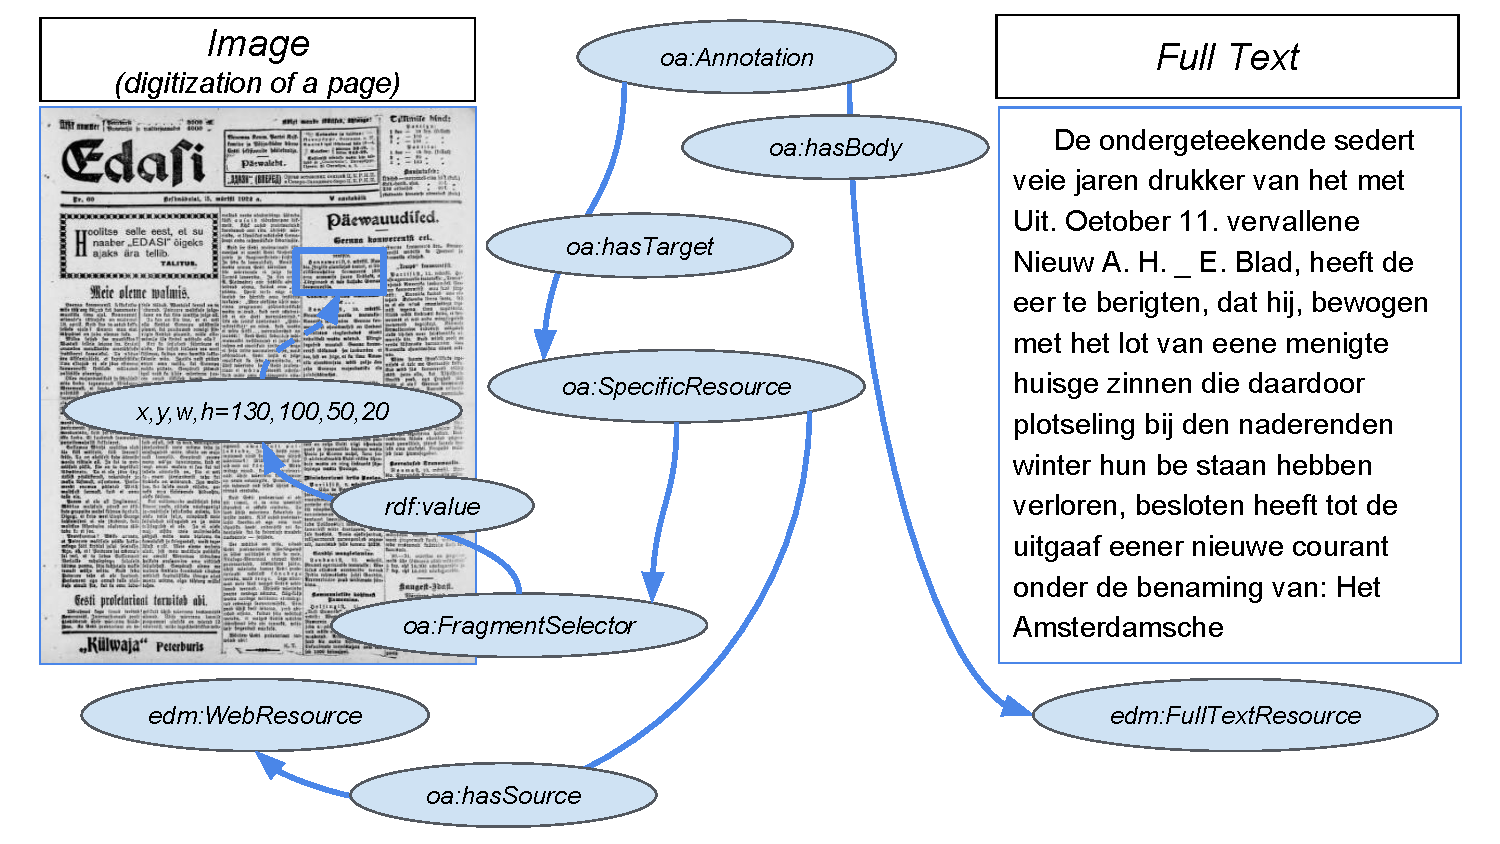
\includegraphics{Fig3}
    \caption{Full-text resource with position on the image.}\label{fig:withposition}
\end{figure}

Our earlier analysis of newspapers corpora \cite{Charles16} has shown that full-text is sometimes represented as several fragments of text, each referring to a specific area of an image (an article, a specific line in the text or a word). In this case, the full-text fragment is accompanied with coordinates indicating its position on the image. 

To support this requirement, we introduce in the model the \verb+oa:SpecificResource+ that ``is used in between the Annotation and the body or target, as appropriate, to capture the additional description of how it is used in the annotation'' \cite{Goosen17}. An \verb+oa:FragmentSelector+ is applied as selector within the \verb+oa:SpecificResource+ to restrict the original target (the \verb+edm:WebResource+) to the specific area to which the text, or fragment, corresponds. Figures \ref{fig:withposition}, \ref{fig:fragmentselector} and \ref{fig:textpositionselector} show examples of this solution.

In Figure~\ref{fig:withposition}, the \verb+edm:FullTextResource+ consists of a fully-fledged resource that corresponds to a paragraph whose position is indicated by the \verb+oa:FragmentSelector+. Note that for rectangle areas, coordinates in the \verb+oa:FragmentSelector+ must follow the Media Fragments W3C recommendation and be the subject of a \verb+dcterms:conformsTo+ statement referring to \url{http://www.w3.org/TR/media-frags/} (not shown in the figure).

\subsubsection{Full-text selections represented as fragments with a position in the image}

\begin{figure}
    \centering
    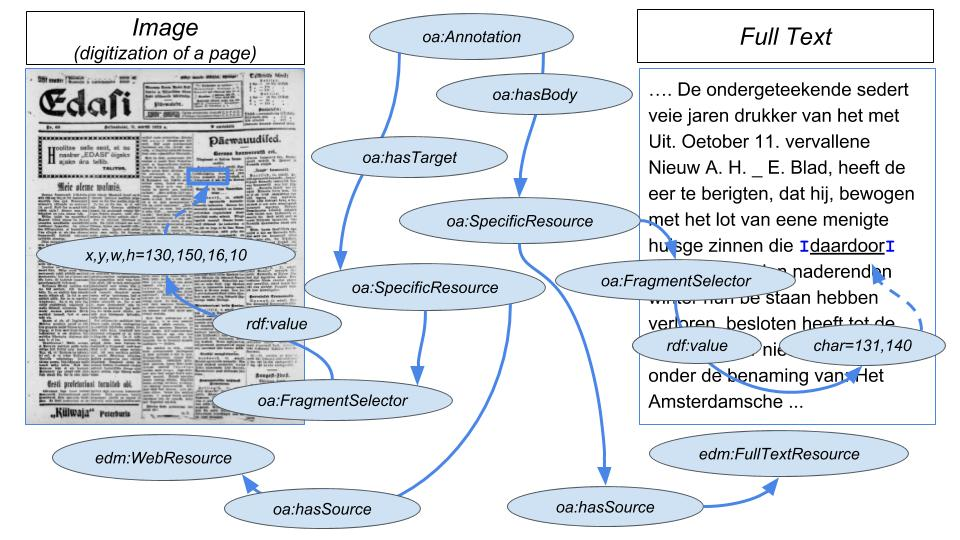
\includegraphics{Fig4}
    \caption{Full-text fragment with position on the image using \emph{oa:FragmentSelector}.}\label{fig:fragmentselector}
\end{figure}

\begin{figure}
    \centering
    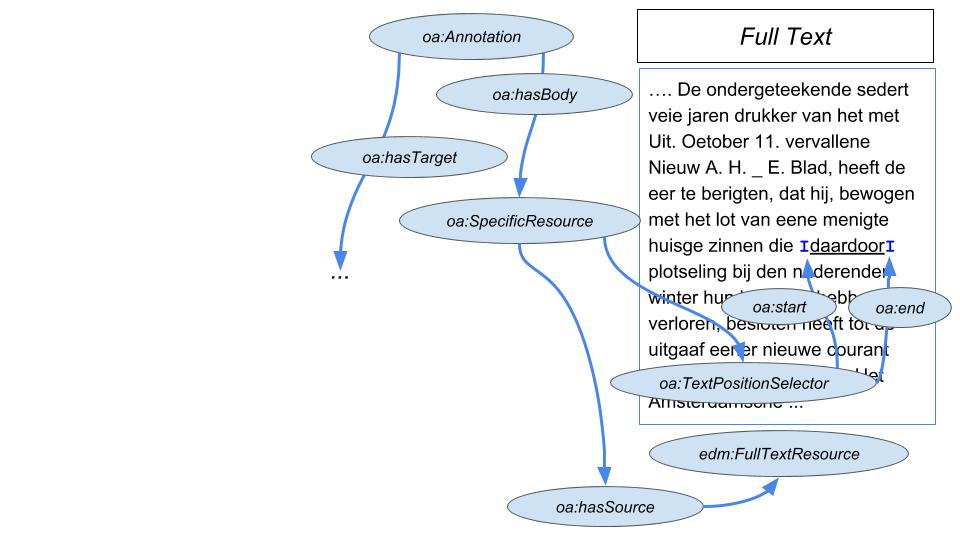
\includegraphics{Fig5}
    \caption{Full-text fragment with position using \emph{oa:TextPositionSelector}.}\label{fig:textpositionselector}
\end{figure}

Figure~\ref{fig:fragmentselector} shows how more details – in this case, the position of a particular word –  can be specified for the association between full-text and images. The area is indicated using the pattern already seen in Figure~\ref{fig:withposition}, but the paragraph fragment that corresponds to the word in the full-text is also given: an \verb+oa:SpecificResource+ is created to represent how the textual body of the annotation is derived from another resource. An \verb+oa:FragmentSelector+ resource describes the range of text by recording the first and last characters' positions within the source. The \verb+oa:FragmentSelector+ must follow RFC 5147 and be the subject of a dcterms:conformsTo statement referring to http://tools.ietf.org/rfc/rfc5147 (not shown in Figure~\ref{fig:fragmentselector}). Note that the WA model offers alternatives for representing fragments: e.g., for text fragments, the data from Figure~\ref{fig:fragmentselector} can also be represented using an \verb+oa:TextPositionSelector+, recording the start and end positions with specific properties (see Figure~\ref{fig:textpositionselector}). We have decided for now to be flexible in what Europeana will accept, opening the possibility to use equivalent WA selectors. But we will seek to normalize the data we publish, i.e. retaining only one of the options – yet to be discussed with the community.

\subsubsection{Logical structure of the full-text}

\begin{figure}
    \centering
    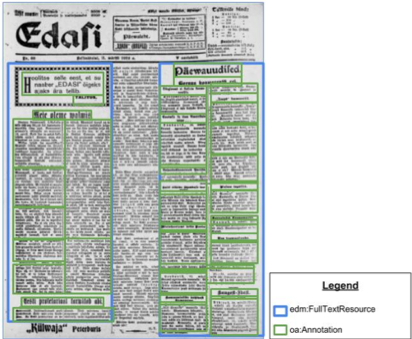
\includegraphics{Fig6}
    \caption{Representing the logical structure of articles and paragraphs of full-text with \emph{edm:FullTextResource} and \emph{oa:Annotation}.}\label{fig:logialstructure}
\end{figure}

Some digitization efforts apply segmentation techniques to detect the independent sections (such as articles) within a newspaper page. Our EDM extension allows representing the different sections in the full-text. First, text of different levels can be represented as different \verb+edm:FullTextResources+ connected across levels using Dublin core dcterms:hasPart and dcterms:isPartOf properties. EDM allows this for any digital representation, and this pattern can be used in particular between a newspaper file that contains several pages (images) and the image of each page. In this case, however, text is duplicated across levels. An alternative is to represent the logical structure via the organization of \verb+edm:FullTextResources+ and \verb+oa:Annotations+. Our extension assumes that each \verb+edm:FullTextResource+ can reflect a section within a page and act as  grouping for all related \verb+oa:Annotations+. Figure~\ref{fig:logialstructure} shows a newspaper page where two \verb+edm:FullTextResources+ represent two articles in the page. It also highlights how (targets of) \verb+oa:Annotations+ represent the paragraphs within each \verb+edm:FullTextResource+.

\subsubsection{Specifying the language of the full-text}

\begin{figure}
  \begin{subfigure}[t]{0.5\textwidth}
    \centering
    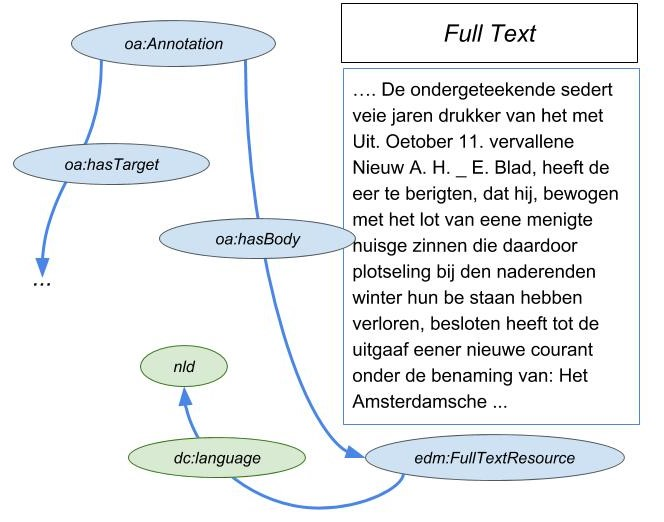
\includegraphics[width=0.8\textwidth]{Fig7a}
    \caption{for the whole \emph{edm:FullTextResource}}
  \end{subfigure}\hfill
  \begin{subfigure}[t]{0.5\textwidth}
    \centering
    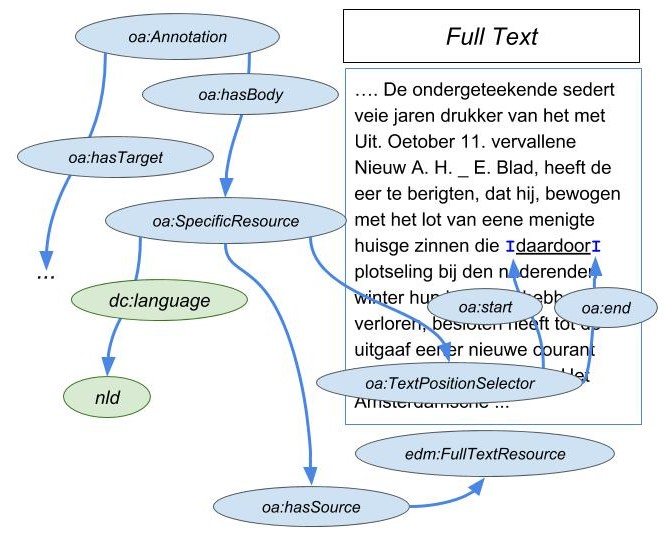
\includegraphics[width=0.8\textwidth]{Fig7b}
    \caption{for a piece of text in isolation (i.e., a word)}
  \end{subfigure}
  \caption{Specification of the language of the text.}\label{fig:example}\label{fig:languagespecification}
\end{figure}

The profile allows the indication of language of the full-text at several levels of detail. At the most general level, the language indicated in the data for the original cultural object (using Dublin Core's dc:language property on EDM's \verb+edm:ProvidedCHO+
resource\footnote{\verb+ProvidedCHO+ stands for `Provided Cultural Heritage Object'. It is the original object that is described. It may be either a physical object (painting, book, etc.) or digital-born object.})
can be seen to apply to the whole full-text as well. Our profile assumes that when a (sub-component of) the full-text does not specify its language, then it inherits the language from the higher levels of its hierarchy. This pattern enables to represent cases when a word in one language is present within a text in another language. But there can be different languages, or a data publisher may prefer to express precise information that does not depend on implicit `propagation' rules between levels in the data. Therefore, the language may be specified at the level of any \verb+edm:FullTextResource+, using an RDF language tag on the \verb+rdf:value+ of the resource or the dc:language property\footnote{Here again there are two equivalent modeling alternatives: the `traditional’ RDF one (already used in EDM and one preferred by the WA model. We intend to accept both and publish both in parallel, but this choice is still open to community feedback.}.
At the finest level of detail, languages may be specified on the oa:SpecificResource referring to text fragments. Figure~\ref{fig:languagespecification} illustrates using dc:language on the \verb+edm:FullTextResource+ and the \verb+oa:SpecificResource+.

\section{Future Work and Conclusion}
\label{sec:conclusion}

Europeana's investigations in exploring its newspapers full-text corpus with research infrastructures has provided valuable input for making CH corpora better discoverable, accessible, machine processable and citable in research contexts. The requirements identified for research usage of CH full-text corpora support several aspects of the current strategy of Europeana towards improving data quality and direct access to the media contents of CH digital objects \cite{publishingGuide}. 

The currently aggregated full-text corpus of Europeana Newspapers has not grown since the end of the Europeana Newspapers project, and an aggregation process based on the ALTO profile was impossible to establish in a sustainable way at Europeana. The new model, being based on EDM and following the IIIF Community approach is expected to lower the technical barriers to establish a sustainable full-text aggregation process. Currently, Europeana is already converting the Europeana Newspapers corpus to the EDM full-text profile and adapting its infrastructure for ingestion of the corpus . In the near future, our EDM full-text profile is going to be used as the basis to re-start the aggregation processes of full-text newspapers content across the Europeana Network. In parallel, we will update the EDM full-text profile, by devising a more precise approach to the modeling alternatives that the current version allows – we have already begun to actively seek feedback from the IIIF Newspapers community. We will also tackle new requirement that could emerge during its adoption: for example, some Europeana stakeholders have voiced interested in an explicit representation of the granularity of the full-text (page, article, paragraph, line, word).

Future work will also address the indexing and retrieval of full-text EDM data, as well as the evaluation of its capacity for supporting rich user-interfaces and data re-use through Europeana's APIs as well as through research infrastructures.

%%
%% Bibliography
%%

%% Please use bibtex, 

\bibliography{oasics-v2019-sample-article}

\end{document}
